In this chapter, we examine the effect of including tetraquark operators on the spectrum in the scalar meson sectors containing the $K_0^*(700)$ (here and often elsewhere referred to as the $\kappa$) and the $a_0(980)$ in $N_f = 2 + 1$ QCD, using an anisotropic lattice with gauge field configurations generated by the Hadron Spectrum Collaboration~\cite{}. It has been suggested that the $\kappa$ and $a_0(980)$ could have tetraquark content~\cite{Jaffe:2004ph, AMSLER200461, Close_2002, PhysRevLett.93.212002}, and to date, there have been a small number of studies investigating tetraquarks on the lattice using light quarks. In 2010, Prelovsek et al. investigated the $\sigma$ and $\kappa$ as possible tetraquark candidates, but neglected disconnected diagrams in their calculations~\cite{Prelovsek2010}. Using tetraquark interpolators, they found an additional light state in both the $\sigma$ and $\kappa$ channels. In 2013, the ETM collaboration examined the $a_0(980)$ and $\kappa$ using four-quark operators~\cite{Alexandrou2013}, though they also neglected disconnected diagrams in their calculations. They found no evidence of an additional state that can be interpreted as a tetraquark. In 2018, Alexandrou et al. conducted a study of the $a_0(980)$ with four-quark operators~\cite{Alexandrou2018}, including disconnected contributions. In their study, they found an additional finite-volume state in the sector containing the $a_0(980)$ meson, which couples to a diquark-antidiquark interpolating field, in the range of ... to ... Additionally, they conclude that disconnected diagrams have drastic effects on their results, and thus cannot be neglected.

We perform Monte Carlo calculations using $412$ gauge field configurations on an anisotropic ($\frac{a_s}{a_t} \approx 3.451$) lattice of size $32^3\times 256$, with a length of $3.74$ fm and a pion mass of approximately $230$ MeV. We extract two spectra in each symmetry channel: one using a basis of only single- and two-meson operators, and one using a basis that also includes a tetraquark operator selected from hundreds of tetraquark operators which were tested. We find that including a tetraquark operator yields an additional finite-volume state in each symmetry channel: one rangeing from ... to ... in the $\kappa$ channel, and one ranging from ... to ... in the $a_0(980)$ channel. In this work, we use the stochastic LapH method~\cite{slaph} to evaluate all diagrams in our calculations, including \textit{all} disconnected contributions.

% Preliminary results of  additional states found using tetraquark operators are shown, and possible implications of these states are discussed. This is the first work to study the tetraquarks in the $\kappa$ and $a_0(980)$ sectors of $N_f = 2 + 1$, $m_\pi \approx 230$ MeV QCD with proper evaluation of all diagrams in the correlator Wick contractions. Previous studies of the $\kappa$  have invalidly neglected the evaluation of disconnected contributions, and only one $N_f = 2 + 1$ study of the $a_0(980)$ to date, by Alexandrou et al.~\cite{}, has included disconnected diagrams. That study, done at $m_\pi \approx 300$ MeV, identified an additional tetraquark-associated level in the range of 1100 to 1200 MeV, which they claim to be a candidate for the $a_0(980)$ meson. We find an additional state in the range of ... to ...

% It has been suggested that the light scalar mesons $K_0^*(700)$ (here referred to as the $\kappa$) and $a_0(980)$ could have tetraquark content~\cite{Jaffe:2004ph, AMSLER200461, Close_2002, PhysRevLett.93.212002}. To date, there have been a small number of studies investigating tetraquarks on the lattice using light quarks. In 2010, Prelovsek et al. investigated the $\sigma$ and $\kappa$ as possible tetraquark candidates, but neglected disconnected diagrams in their calculations~\cite{Prelovsek2010}. Using tetraquark interpolators, they found an additional light state in both the $\sigma$ and $\kappa$ channels. In 2013, the ETM collaboration examined the $a_0(980)$ and $\kappa$ using four-quark operators~\cite{Alexandrou2013}, though they also neglected disconnected diagrams in their calculations. They found no evidence of an additional state that can be interpreted as a tetraquark. In 2018, Alexandrou et al. conducted a study of the $a_0(980)$ with four-quark operators~\cite{Alexandrou2018}, including disconnected contributions. In their study, they found an additional finite-volume state in the sector containing the $a_0(980)$ meson, which couples to a diquark-antidiquark interpolating field. Additionally, they conclude that disconnected diagrams have drastic effects on their results, and thus cannot be neglected.

% Here we investigate the possible role of tetraquark operators in lattice QCD in the symmetry channels of the $\kappa$ ($I = \frac{1}{2}$, $S=1$, $P = +1$, $J=0$) and $a_0(980)$ ($I=1$, $S=0$, $P=+1$, $G=-1$, $J=0$). We perform Monte Carlo calculations using $412$ gauge field configurations on an anisotropic ($\frac{a_s}{a_t} \approx 3.451$) lattice of size $32^3\times 256$, with a length of $3.74$ fm and a pion mass of approximately $230$ MeV. We extract two spectra in each symmetry channel: one using a basis of only single- and two-meson operators, and one using a basis that also includes a tetraquark operator selected from hundreds of tetraquark operators which were tested. We find that including a tetraquark operator yields an additional finite-volume state in each symmetry channel. In this work, we use the stochastic LapH method~\cite{slaph} to evaluate all diagrams in our calculations, including \textit{all} disconnected contributions.


\section{Operator construction}
We include single- and two- meson operators, as well as tetraquark operators, in the basis of interpolating operators. We construct our elemental operators using building blocks of smeared, gauge-covariantly displaced quark fields, and stout-smeared link variables. To form the final operators out of our elemental operators, we project the elemental operators onto various symmetry channels according to isospin, parity, $G$-parity, octahedral little group, etc. That is, to form a meson operator $M_{l}(t)$ that transforms irreducibly under all symmetries of interest (labeled by the compound index $l$) at time $t$, we must 
take a linear combination of our elemental meson operators, $M_{l}(t)=c_{\alpha \beta}^{(l)} \Phi_{\alpha \beta}^{A B}(\boldsymbol{p}, t)$. To form a two-meson operator $\mathcal{O}_l(t)$, we would follow a similar procedure and project the product of two final meson operators $M^{a}_{l_a}(t) M^{b}_{l_a}(t)$ onto a final symmetry channel $l$: $\mathcal{O}_l(t) = c^{(l)}_{l_a l_b} M^{a}_{l_a}(t) M^{b}_{l_a}(t)$.

In order to construct a tetraquark operator, we must consider the various ways to construct a color-singlet four-quark object out of four quark fields. As seen in Ref.~\cite{pittir33243}, the Clebsch-Gordon decompositions show that the only way to construct a color-singlet is by using two quarks and two antiquarks, and that doing so yields two linearly independent color singlet objects:
\begin{equation}
\begin{array}{l}
    {3 \otimes 3 \otimes 3 \otimes 3=3\oplus3\oplus3\oplus\overline{6}\oplus\overline{6}\oplus15\oplus15\oplus15\oplus15},\\
    {3 \otimes 3 \otimes 3 \otimes \overline{3}=\overline{3}\oplus\overline{3}\oplus\overline{3}\oplus6\oplus6\oplus6\oplus\overline{15}\oplus\overline{15}\oplus24},\\
    {3 \otimes 3 \otimes \overline{3} \otimes \overline{3}=1\oplus1\oplus8\oplus8\oplus8\oplus8\oplus10\oplus\overline{10}\oplus27}.
\end{array}
\end{equation}
There are 81 basis vectors formed by the quark fields, $p_{a}^{*}(x) q_{b}^{*}(x) r_{c}(x) s_{d}(x)$, where each $r$, $s$ transforms as a color vector in the fundamental $3$ irrep, and so, $p^{*}$, $q^{*}$ transform in the $\overline 3$ irrep. We need two linearly independent and gauge-invariant combinations of these to exhaust all possible tetraquark operators. It is easy to see that the following combinations are both linearly independent and gauge-invariant (and thus form our elemental tetraquark operators):
\begin{equation}\label{eq:tsta}
\begin{aligned} T_{S} &=\left(\delta_{a c} \delta_{b d}+\delta_{a d} \delta_{b c}\right) p_{a}^{*}(x) q_{b}^{*}(x) r_{c}(x) s_{d}(x) \\ T_{A} &=\left(\delta_{\alpha c} \delta_{b d}-\delta_{\alpha d} \delta_{b c}\right) p_{\alpha}^{*}(x) q_{b}^{*}(x) r_{c}(x) s_{d}(x).\end{aligned}
\end{equation}
These elemental tetraquark operators are combinations of two gauge-invariant quark-antiquark constituents. The individual constituents are \textit{not} mesons since they separately do not have well-defined quantum numbers. In other words, we project the entire elemental tetraquark operator onto relevant symmetry channels, rather than each individual quark-antiquark operator.

While we chose only a handful of tetraquark operators for our final analysis, we designed hundreds of operators with differing flavor structures and displacements. We tested these operators by individually adding them to a basis of single- and multi-meson operators to see if an additional level was found. Most of the operators did not yield an additional level, but we found particular operators that did. In the $\kappa$ channel, we tested the following flavor structures: $\overline s u \overline s s$, $\overline s u \overline u u$, $\overline s u \overline d u$. We found that only operators with the $\overline s u \overline s s$ flavor structure yielded an additional finite-volume state. We tested both single-site and quadruple displacements, and found operators of both types that yielded additional finite-volume states. The quadruply-displaced operators came at a higher computational cost and offered no improvements, and so were excluded from the final operator sets. In the $a_0(980)$ channel, we tested the following flavor structures: $\overline u u \overline d u$, $\overline s s \overline d u$, $\overline d u \overline d u$. We found that only operators with the $\overline u u \overline d u$ flavor structure yielded an additional finite-volume state. We only tested single-site operators in the $a_0(980)$ channel, after finding no improvement with other displacement types in the $\kappa$ channel. We also constructed operator bases that included several tetraquark operators, and found that the number of additional levels in the energy range we examined was unchanged.
\section{Lattice Spectra Results (Preliminary)}
\subsection{$\kappa$ Channel}
We summarize results obtained by fitting a spectrum in the $\kappa$ at-rest symmetry channel for two operator bases: one including only single-meson and two-meson operators, and one including single-meson, two-meson, and tetraquark operators. Figure \ref{fig:kappa_spectrum} shows the spectrum with and without the inclusion of a tetraquark operator in the basis. The tetraquark operator is of the flavor structure $\overline s u \overline s s$, is of the antisymmetric form in Eq.~(\ref{eq:tsta}), and has no quark displacement. We found that single-site ($\boldsymbol{d_\alpha} = \boldsymbol{d_\beta} = 0$) tetraquark operators resulted in better (less noisy) correlator signals than displaced operators. We see that including a tetraquark operator yields an additional finite-volume state in the range of $(2.178 - 2.256) m_K$, which is not present when only single- and two-meson operators are used. Additionally, a plot of the overlap factors for the tetraquark operator (Figure~\ref{fig:zkappa}) shows significant overlap onto this extra state (level 3 in the plot). This suggests that there is a finite-volume state in our lattice spectrum that shares quantum numbers with the $\kappa$ resonance, and that has tetraquark content. Whether or not this is evidence of the $\kappa$ resonance having tetraquark content, however, will have to wait for future scattering studies using Lüscher's method.
\begin{figure}
  \hspace{-0.4 in}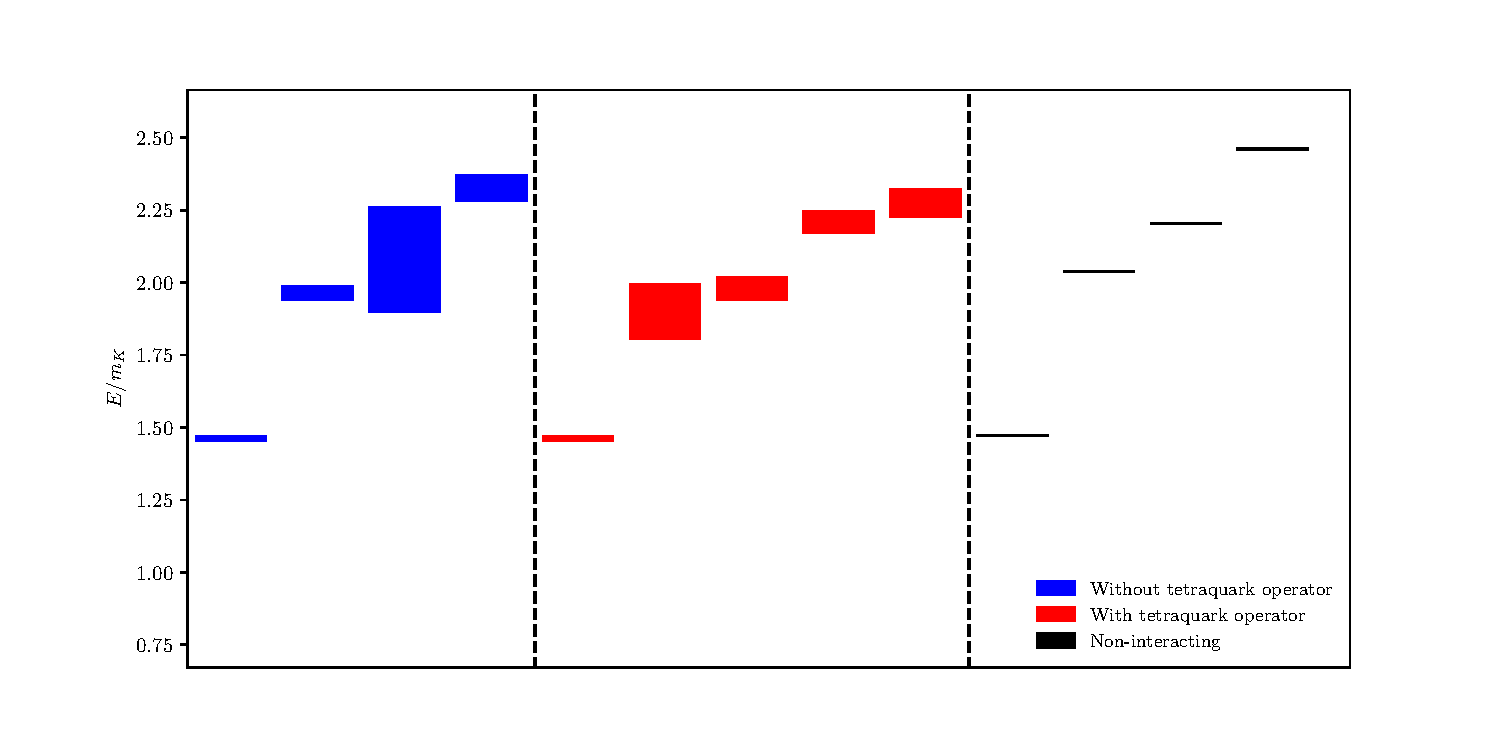
\includegraphics[scale=0.7]{figures/a1g_staircase.pdf}
  \caption{The first five and six levels of the spectrum in the $\kappa$ at-rest symmetry channel. On the left: the spectrum obtained using a basis with no tetraquark operators. In the middle: the spectrum obtained using one tetraquark operator. On the right: non-interacting levels shown for reference, where $(\boldsymbol{d}^2)$ denotes particles with squared momentum $(2\pi\boldsymbol{d}/L)^2$.}\label{fig:kappa_spectrum}
\end{figure}
\begin{figure}
  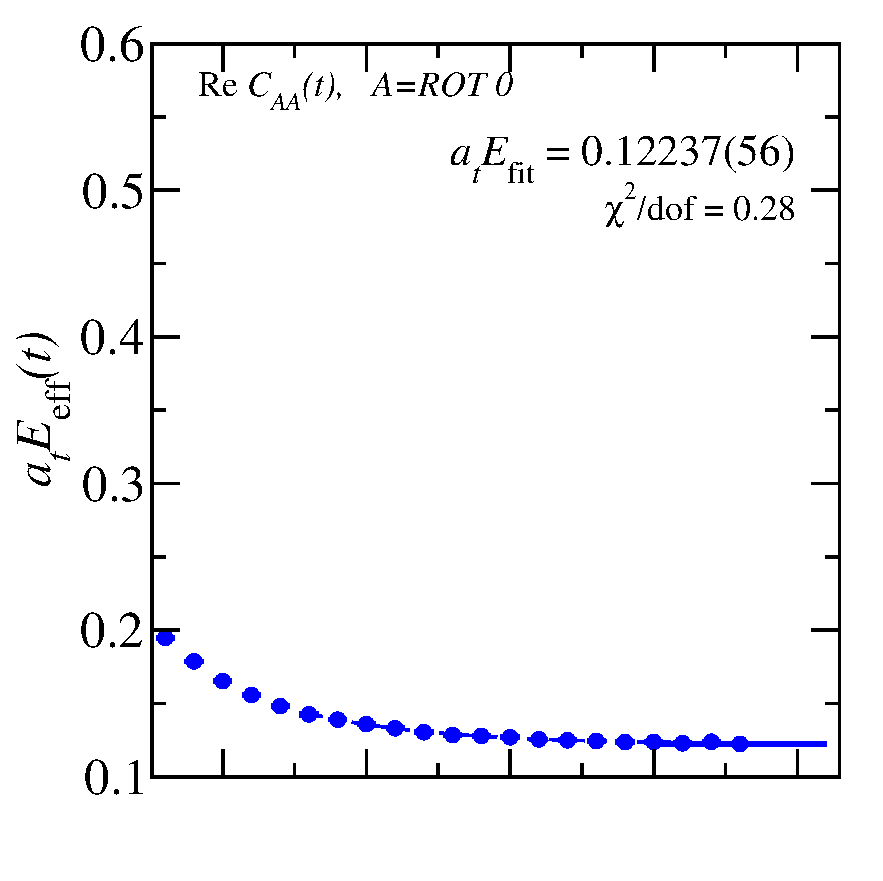
\includegraphics[width=0.318\textwidth]{fits_suss2p_SS4/fit_isodoublet-S1-P000-A1g_1-ROT-0_21000A1g_1-ROT-0T8-26_4.pdf}
  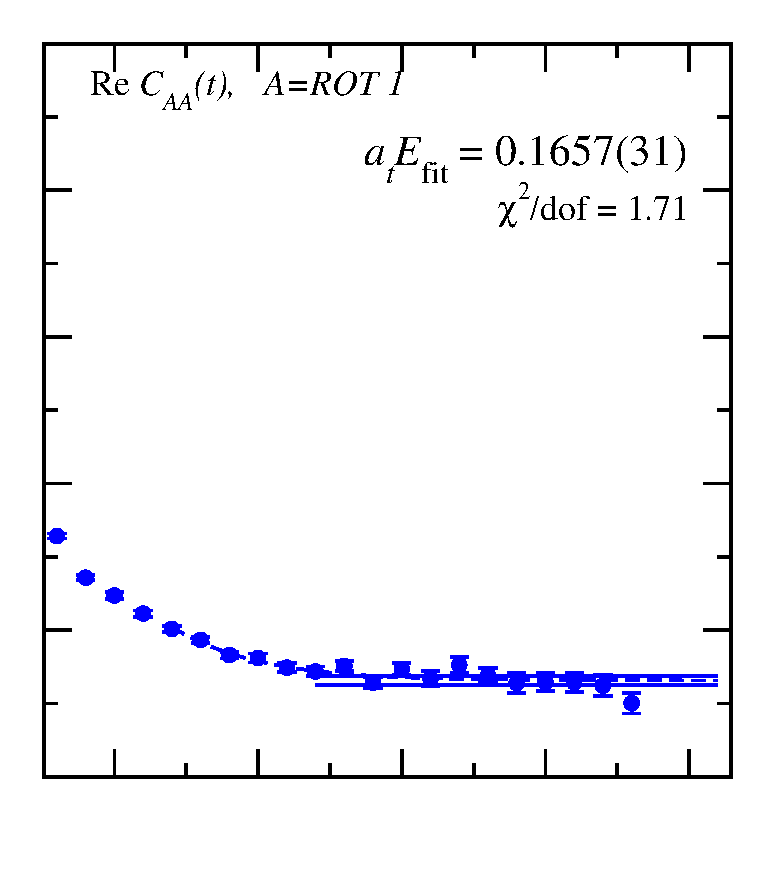
\includegraphics[width=0.28\textwidth]{fits_suss2p_SS4/fit_isodoublet-S1-P000-A1g_1-ROT-1_21000A1g_1-ROT-1T7-26_4.pdf}
  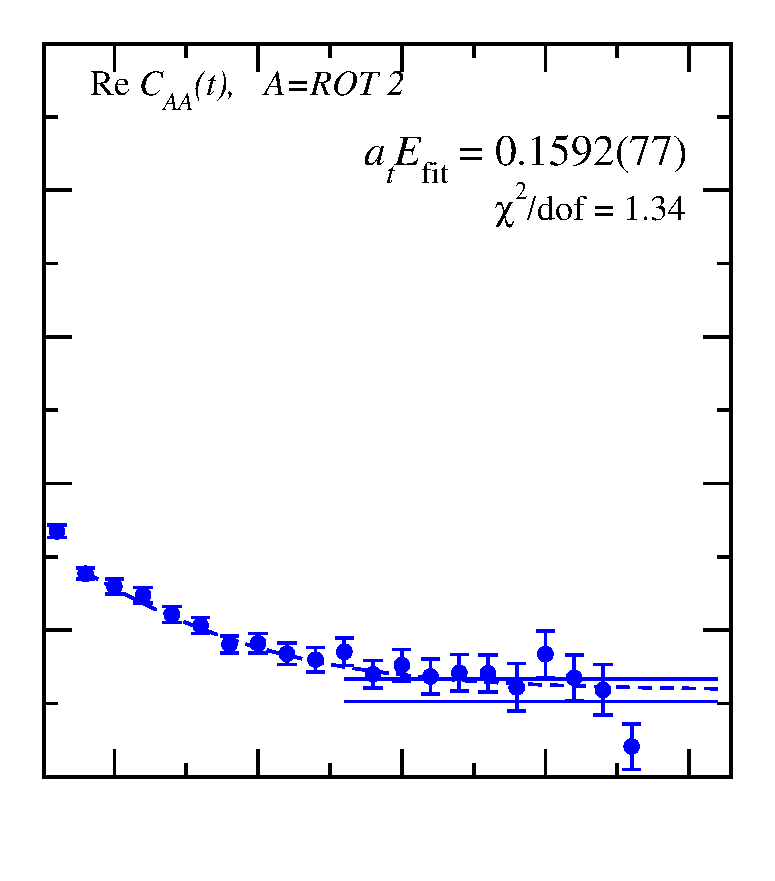
\includegraphics[width=0.28\textwidth]{fits_suss2p_SS4/fit_isodoublet-S1-P000-A1g_1-ROT-2_21000A1g_1-ROT-2T4-26_4.pdf}\\
  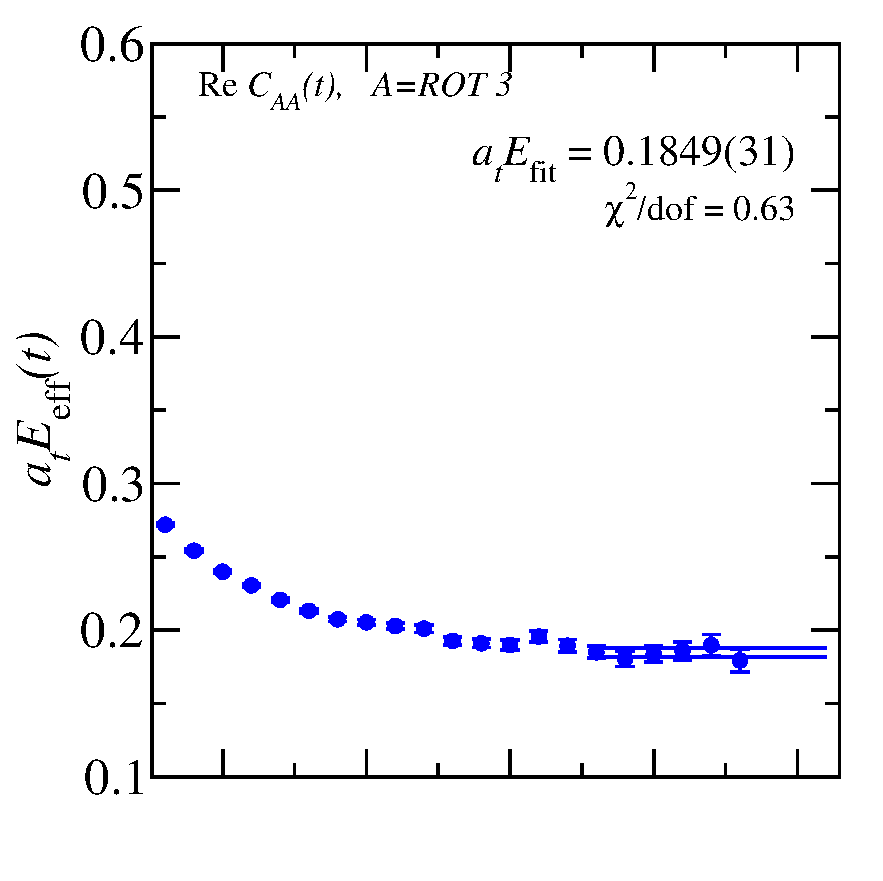
\includegraphics[width=0.318\textwidth]{fits_suss2p_SS4/fit_isodoublet-S1-P000-A1g_1-ROT-3_21000A1g_1-ROT-3T18-26_0.pdf}
  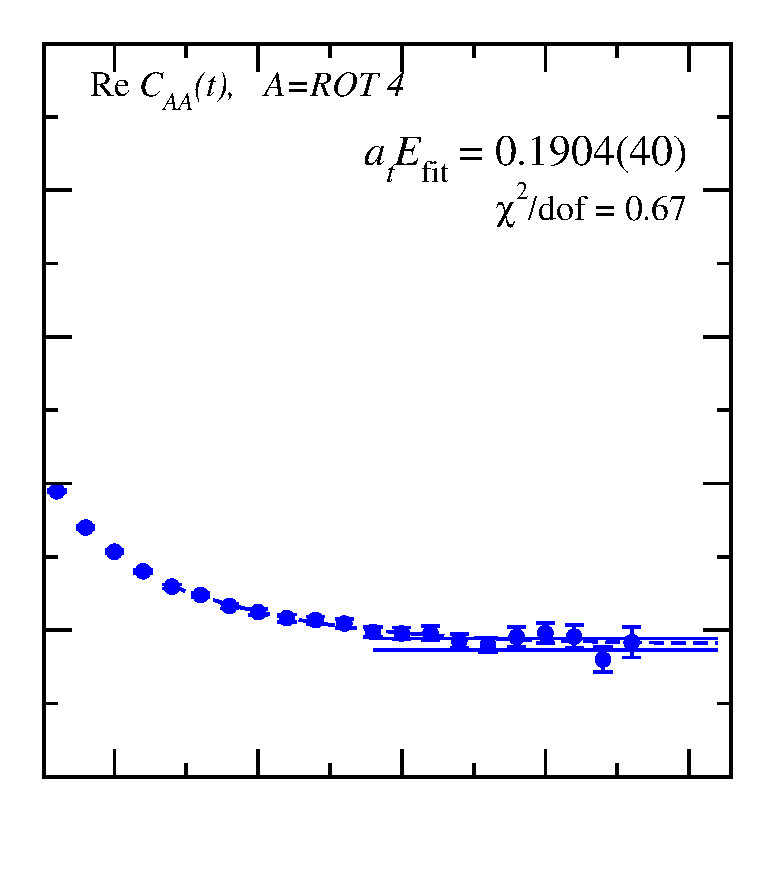
\includegraphics[width=0.28\textwidth]{fits_suss2p_SS4/fit_isodoublet-S1-P000-A1g_1-ROT-4_21000A1g_1-ROT-4T7-26_4.pdf}
  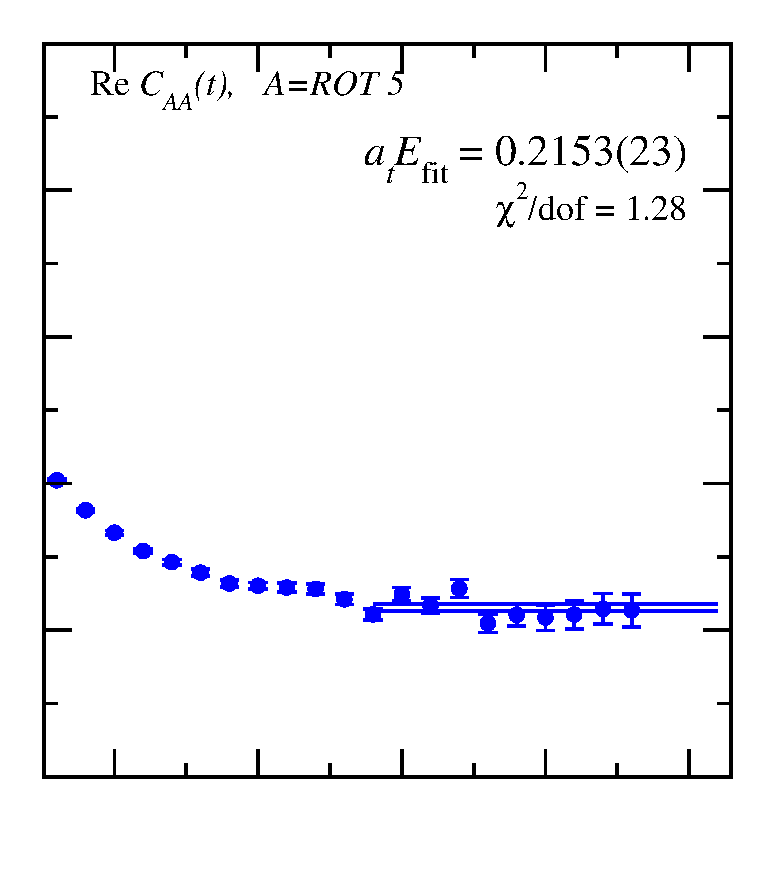
\includegraphics[width=0.28\textwidth]{fits_suss2p_SS4/fit_isodoublet-S1-P000-A1g_1-ROT-5_21000A1g_1-ROT-5T14-26_0.pdf}\\
  \raisebox{0.1in}{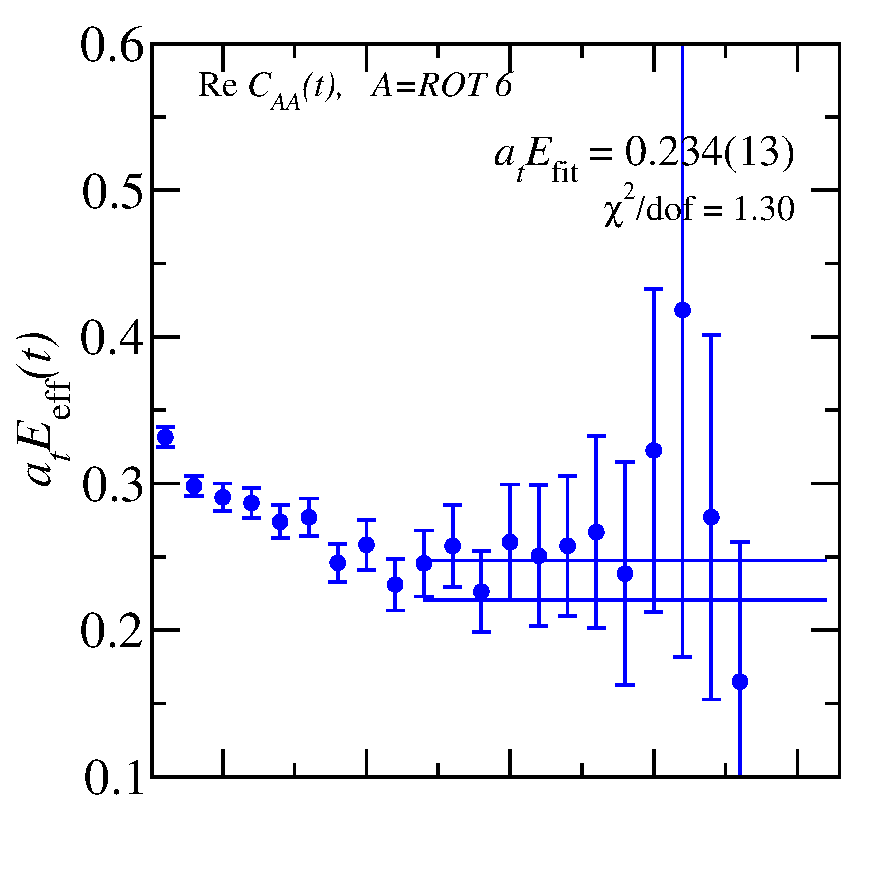
\includegraphics[width=0.318\textwidth]{fits_suss2p_SS4/fit_isodoublet-S1-P000-A1g_1-ROT-6_21000A1g_1-ROT-6T12-26_0.pdf}}
  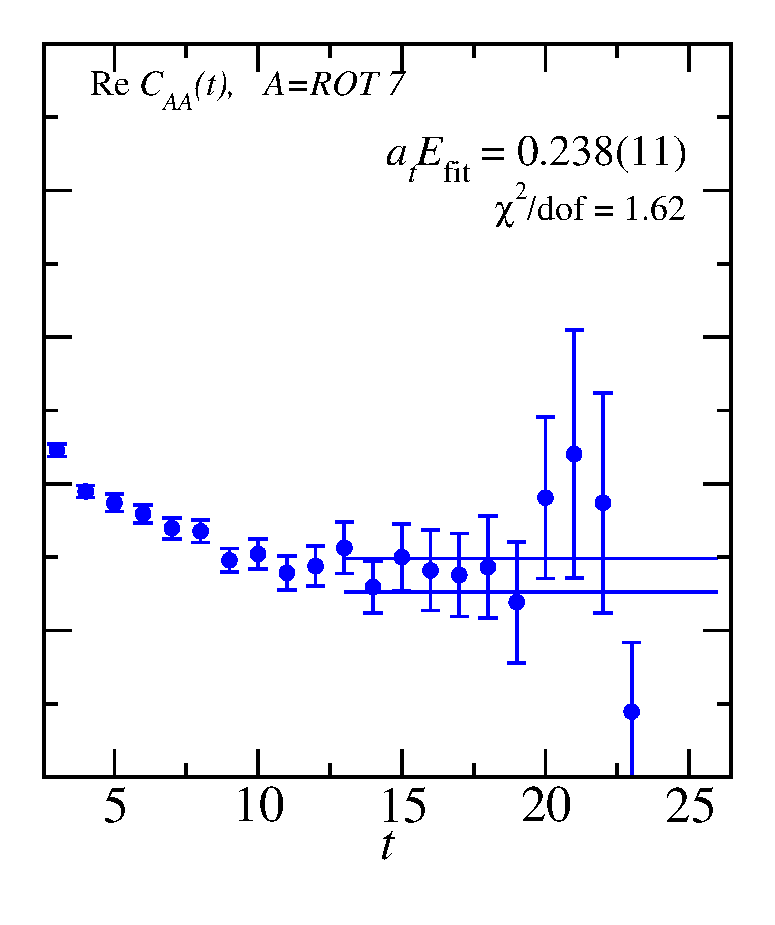
\includegraphics[width=0.28\textwidth]{fits_suss2p_SS4/fit_isodoublet-S1-P000-A1g_1-ROT-7_21000A1g_1-ROT-7T13-26_0.pdf}
  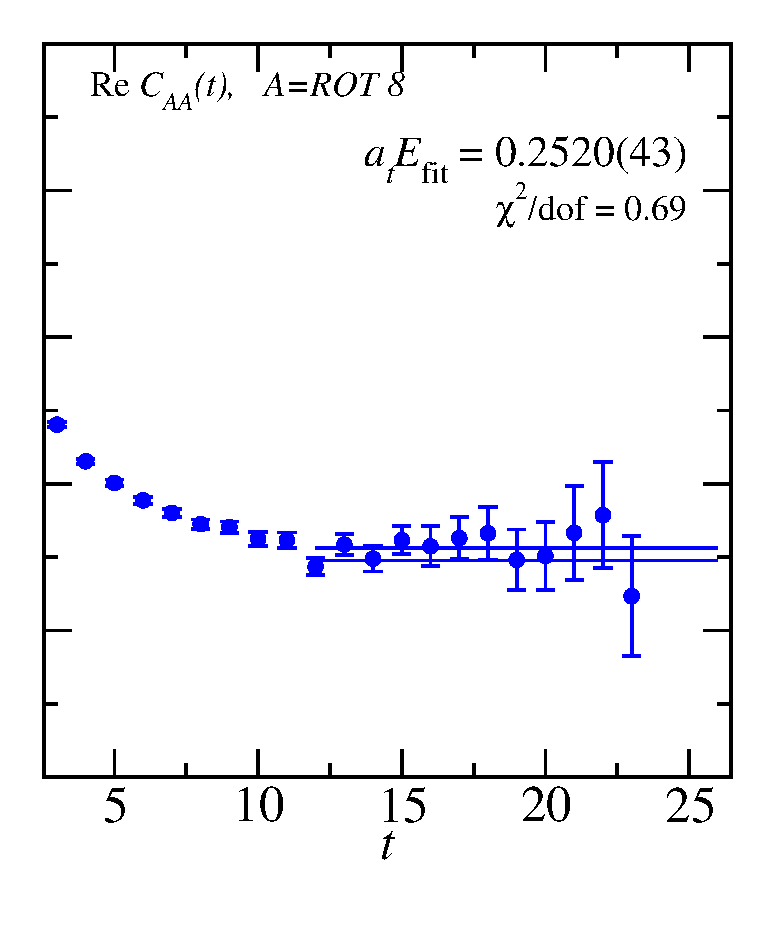
\includegraphics[width=0.28\textwidth]{fits_suss2p_SS4/fit_isodoublet-S1-P000-A1g_1-ROT-8_21000A1g_1-ROT-8T12-26_0.pdf}\\
  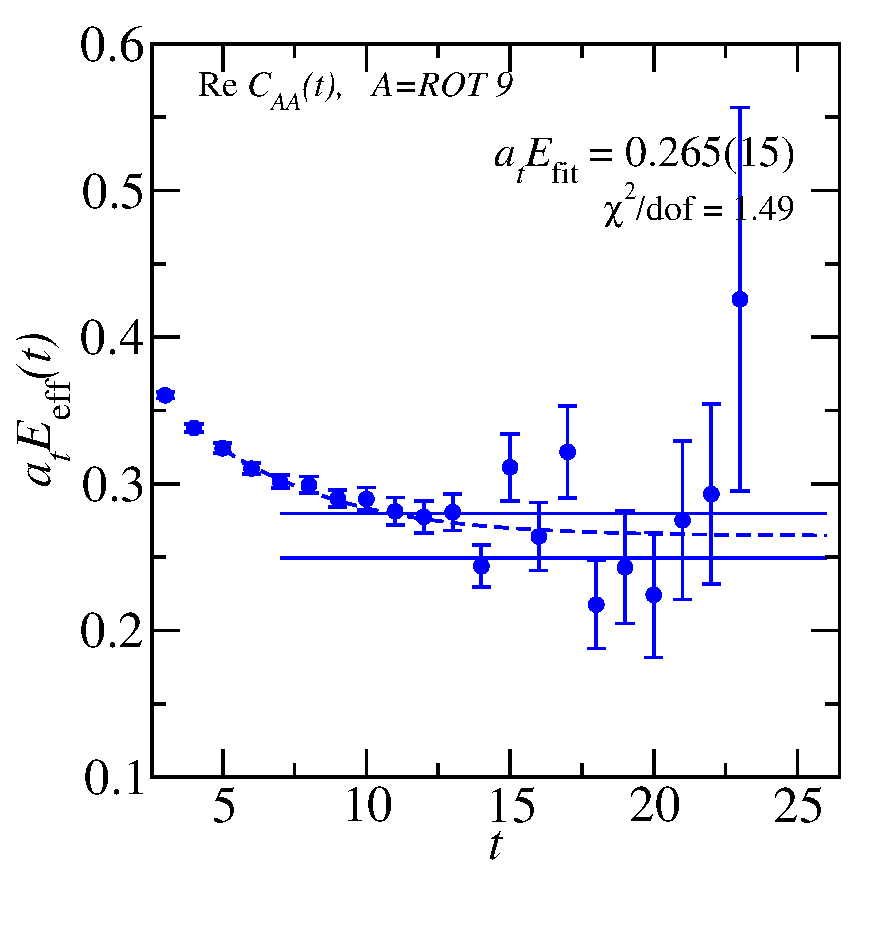
\includegraphics[width=0.318\textwidth]{fits_suss2p_SS4/fit_isodoublet-S1-P000-A1g_1-ROT-9_21000A1g_1-ROT-9T5-26_4.pdf}
  \caption{Effective energies for the rotated 10x10 correlator matrix in the $\kappa$ channel. Effective energy curves calculated from correlator fits are overlaid, and fit results are shown.}\label{fig:kappa_tq_grid}
\end{figure}

\begin{figure}
  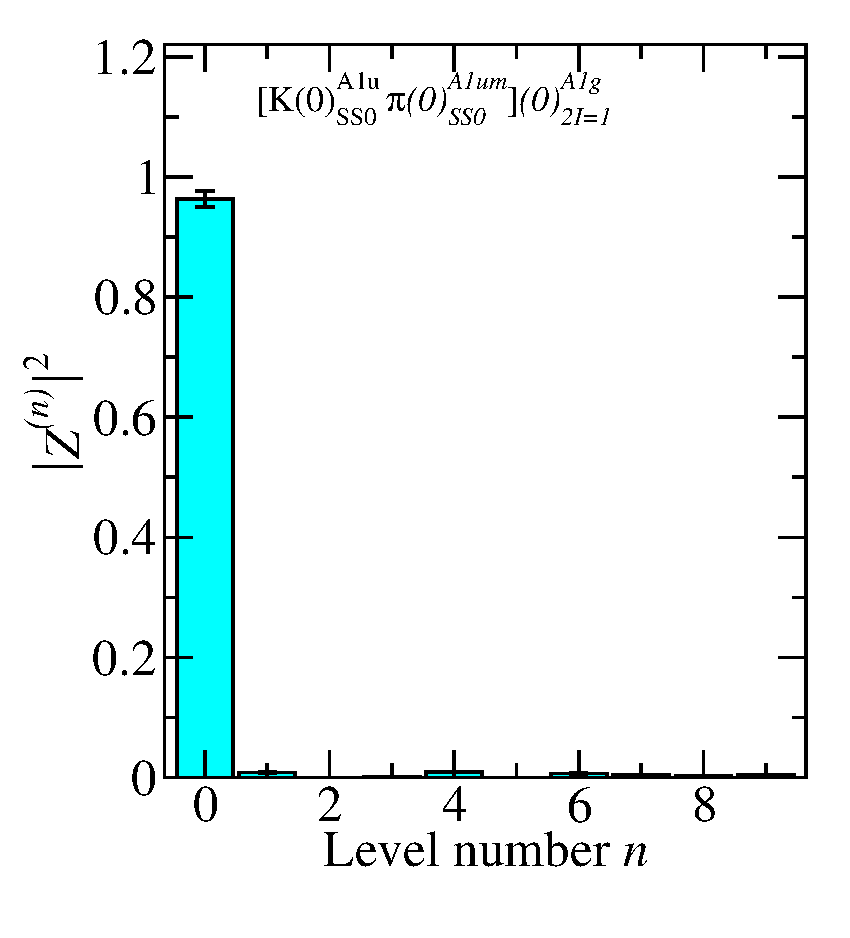
\includegraphics[width=0.3\textwidth]{fits_suss2p_SS4/zfactors/zfactor_isodoublet_kaon_pion-A1g_1-P000-A1u-SS_0-P000-A1um-SS_0.pdf}
  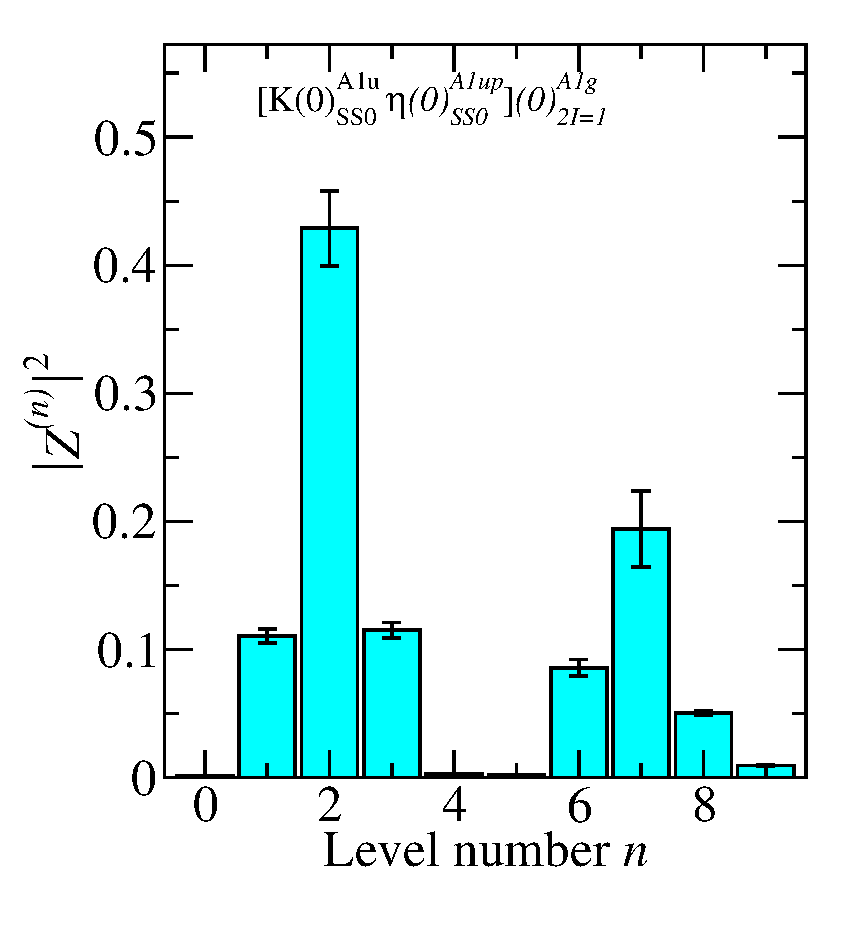
\includegraphics[width=0.3\textwidth]{fits_suss2p_SS4/zfactors/zfactor_isodoublet_kaon_eta-A1g_1-P000-A1u-SS_0-P000-A1up-SS_0.pdf}
  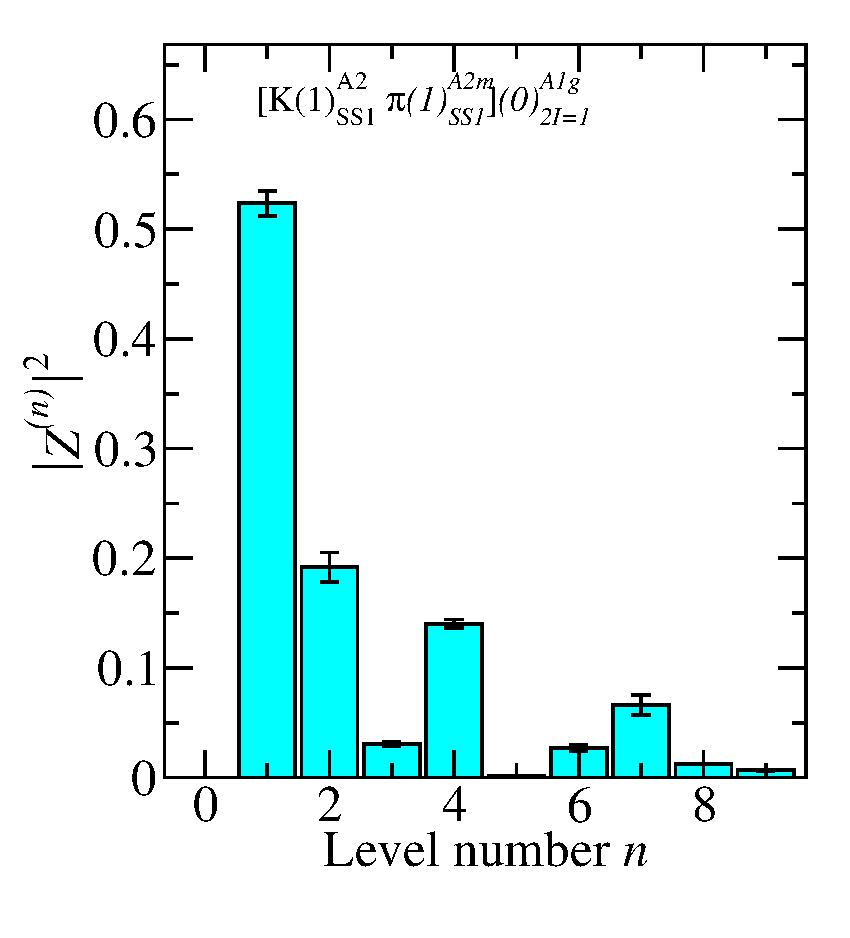
\includegraphics[width=0.3\textwidth]{fits_suss2p_SS4/zfactors/zfactor_isodoublet_kaon_pion-A1g_1-P001-A2-SS_1-P00-1-A2m-SS_1.pdf}\\
  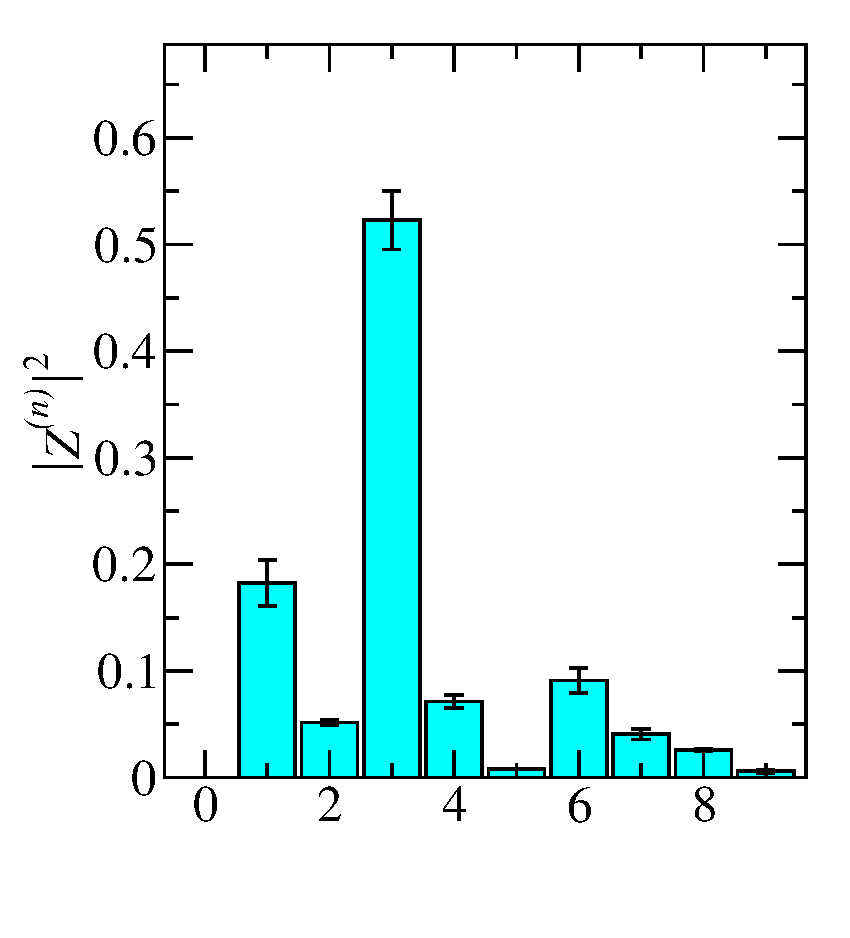
\includegraphics[width=0.3\textwidth]{fits_suss2p_SS4/zfactors/zfactor_tqsuss2p-P000-A1g_1-SS_4.pdf}
  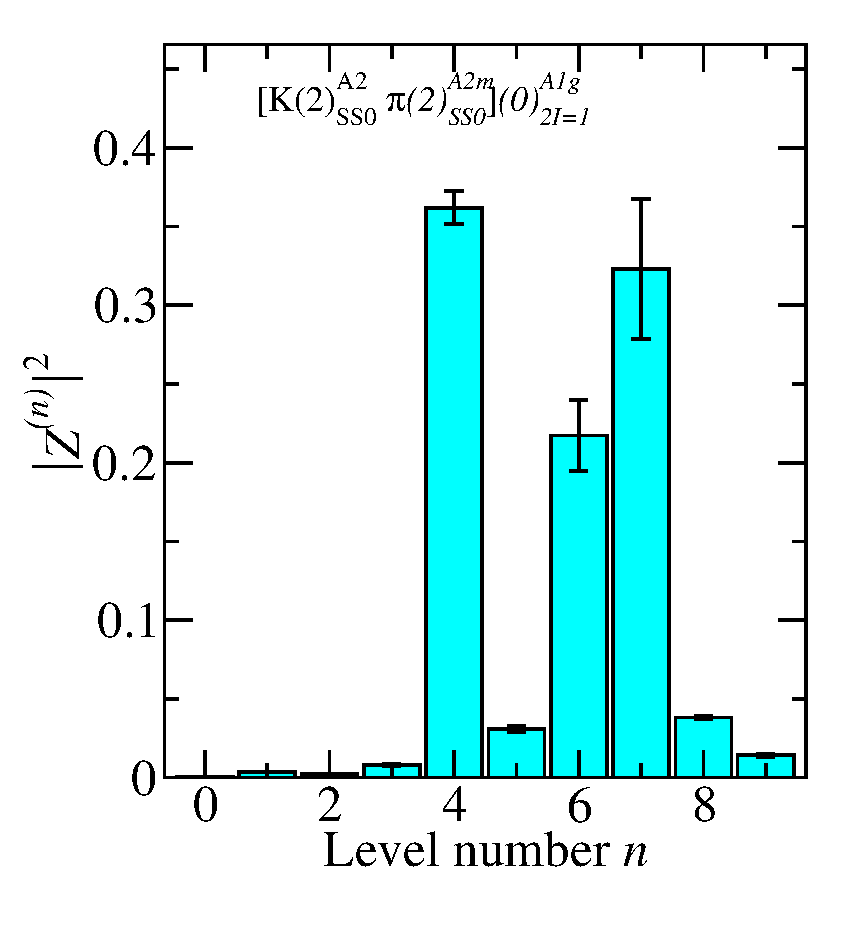
\includegraphics[width=0.3\textwidth]{fits_suss2p_SS4/zfactors/zfactor_isodoublet_kaon_pion-A1g_1-P011-A2-SS_0-P0-1-1-A2m-SS_0.pdf}
  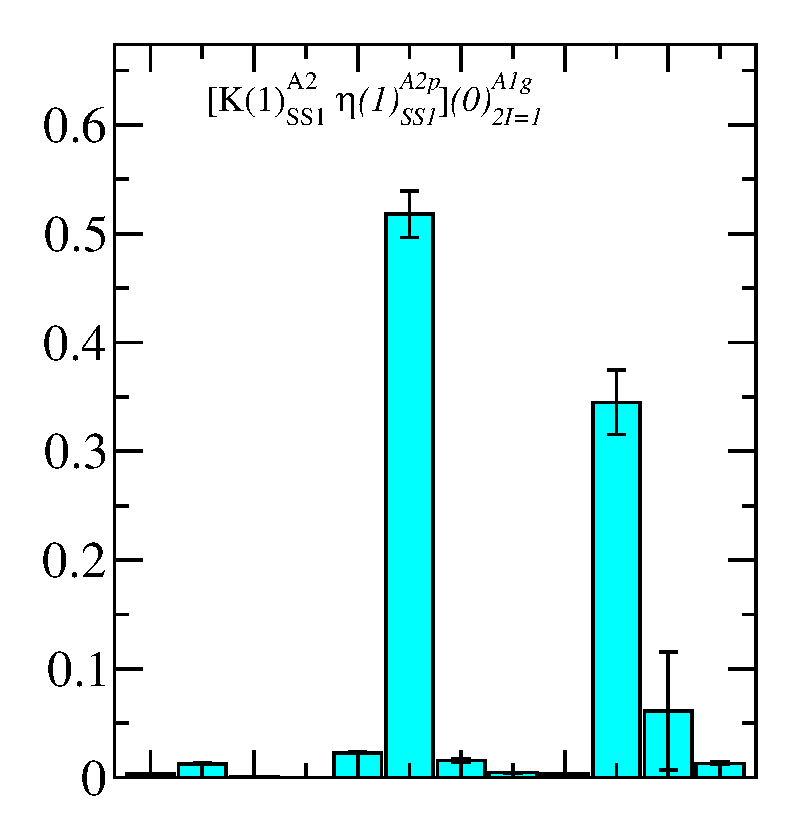
\includegraphics[width=0.3\textwidth]{fits_suss2p_SS4/zfactors/zfactor_isodoublet_kaon_eta-A1g_1-P001-A2-SS_1-P00-1-A2p-SS_1.pdf}\\
  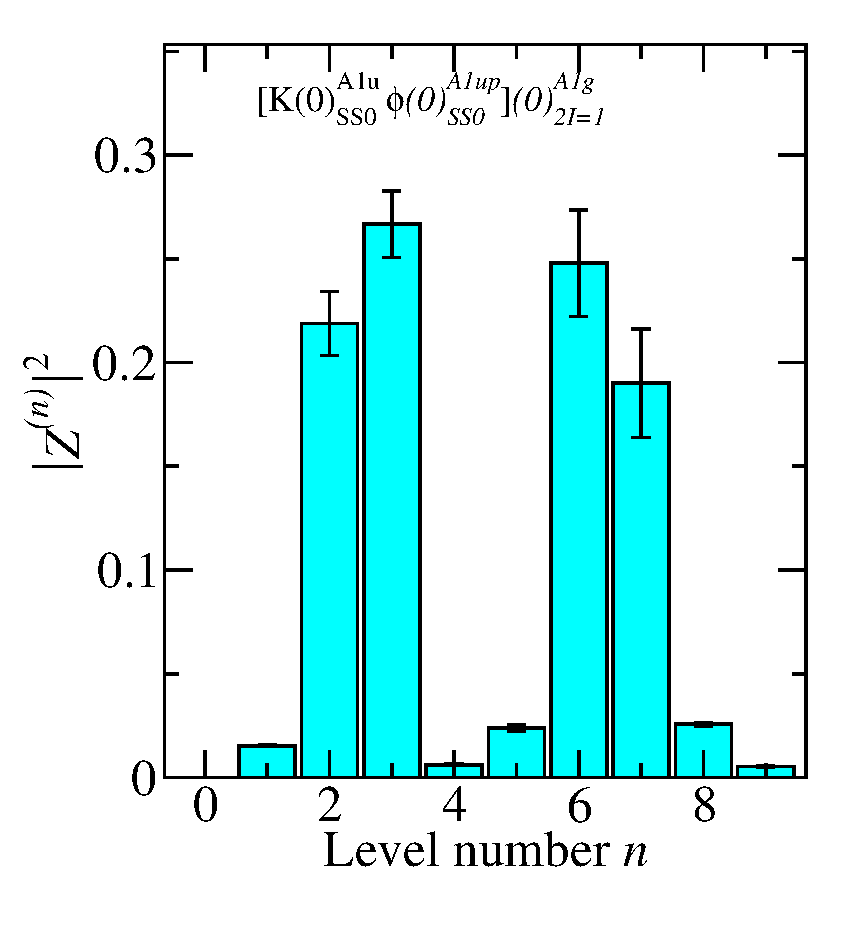
\includegraphics[width=0.3\textwidth]{fits_suss2p_SS4/zfactors/zfactor_isodoublet_kaon_phi-A1g_1-P000-A1u-SS_0-P000-A1up-SS_0.pdf}
  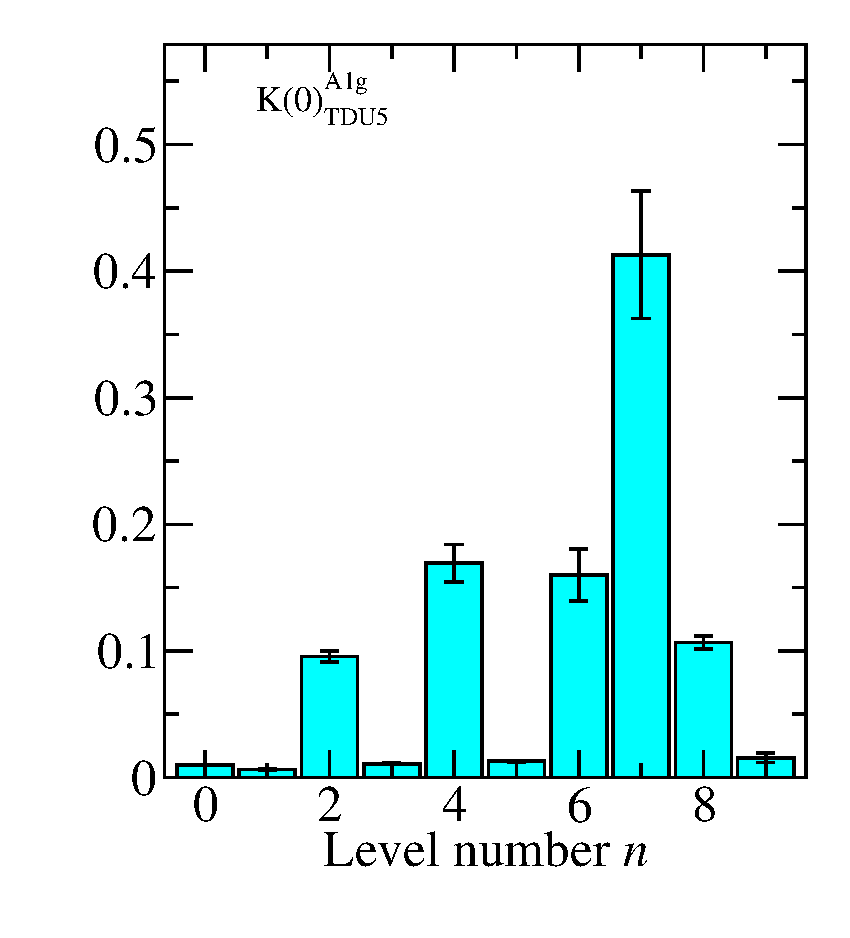
\includegraphics[width=0.3\textwidth]{fits_suss2p_SS4/zfactors/zfactor_kaon-P000-A1g_1-TDU_5.pdf}
  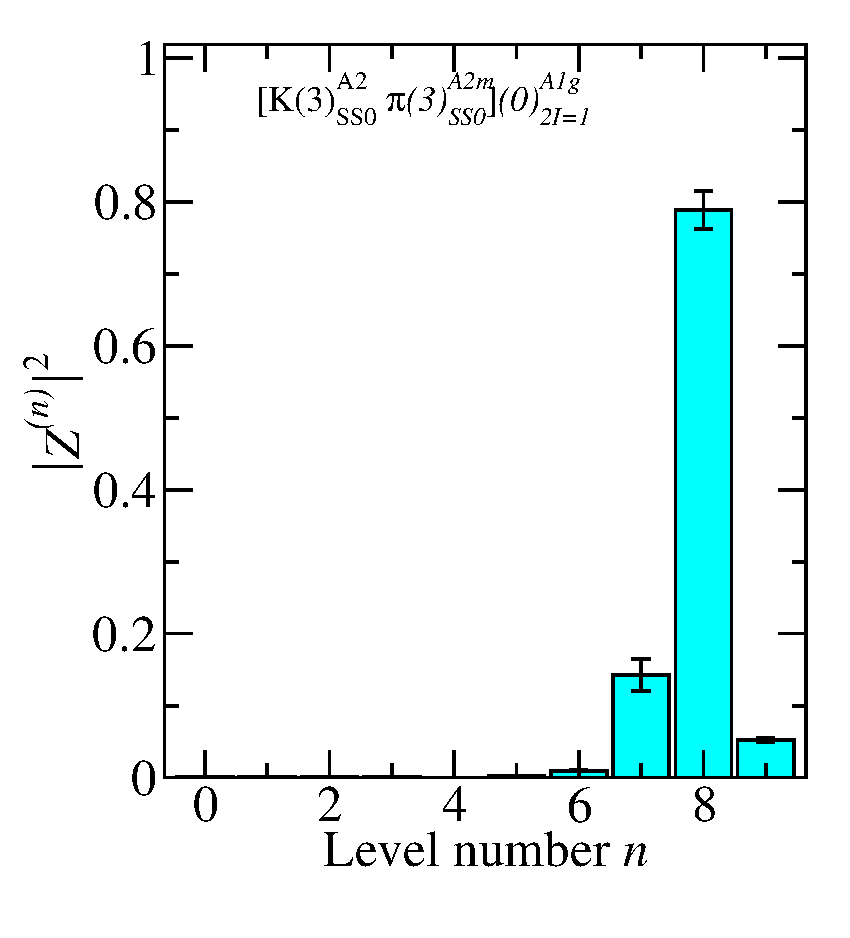
\includegraphics[width=0.3\textwidth]{fits_suss2p_SS4/zfactors/zfactor_isodoublet_kaon_pion-A1g_1-P111-A2-SS_0-P-1-1-1-A2m-SS_0.pdf}\\
  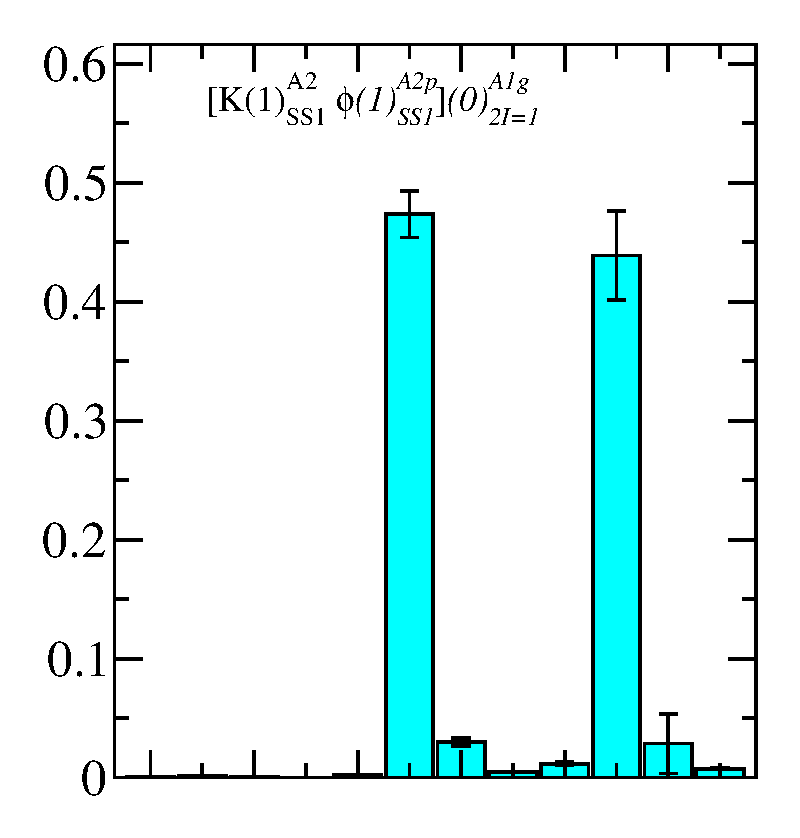
\includegraphics[width=0.3\textwidth]{fits_suss2p_SS4/zfactors/zfactor_isodoublet_kaon_phi-A1g_1-P001-A2-SS_1-P00-1-A2p-SS_1.pdf}
\end{figure}
\subsection{$a_0(980)$ Channel}
We summarize results obtained by fitting a spectrum in the $a_0(980)$ at-rest symmetry channel for again for two operator bases as in the $\kappa$ channel. Figure \ref{fig:a0_spectrum} shows the spectrum with and without the inclusion of a tetraquark operator in the basis. The tetraquark operator is of the flavor structure $\overline u u \overline d u$, is also of the antisymmetric form in (\ref{eq:tsta}), and again has no quark displacement. We again found that using single-site tetraquark operators resulted in better correlator signals than displaced operators. We see an extra level appear in the range of $(2.258 - 2.426) m_K$ when we include a tetraquark operator. Again, overlap factors are shown for the tetraquark operator, and significant overlaps with the additional level (level 3) can be seen in Figure~\ref{fig:za0}. This suggests there is a finite-volume state in our lattice spectrum that shares quantum numbers with the $a_0(980)$ resonance, and that has tetraquark content. As in the $\kappa$-channel case, evidence for or against the $a_0(980)$ having tetraquark content will have to wait for future scattering studies done by applying Lüscher's method.
\begin{figure}
  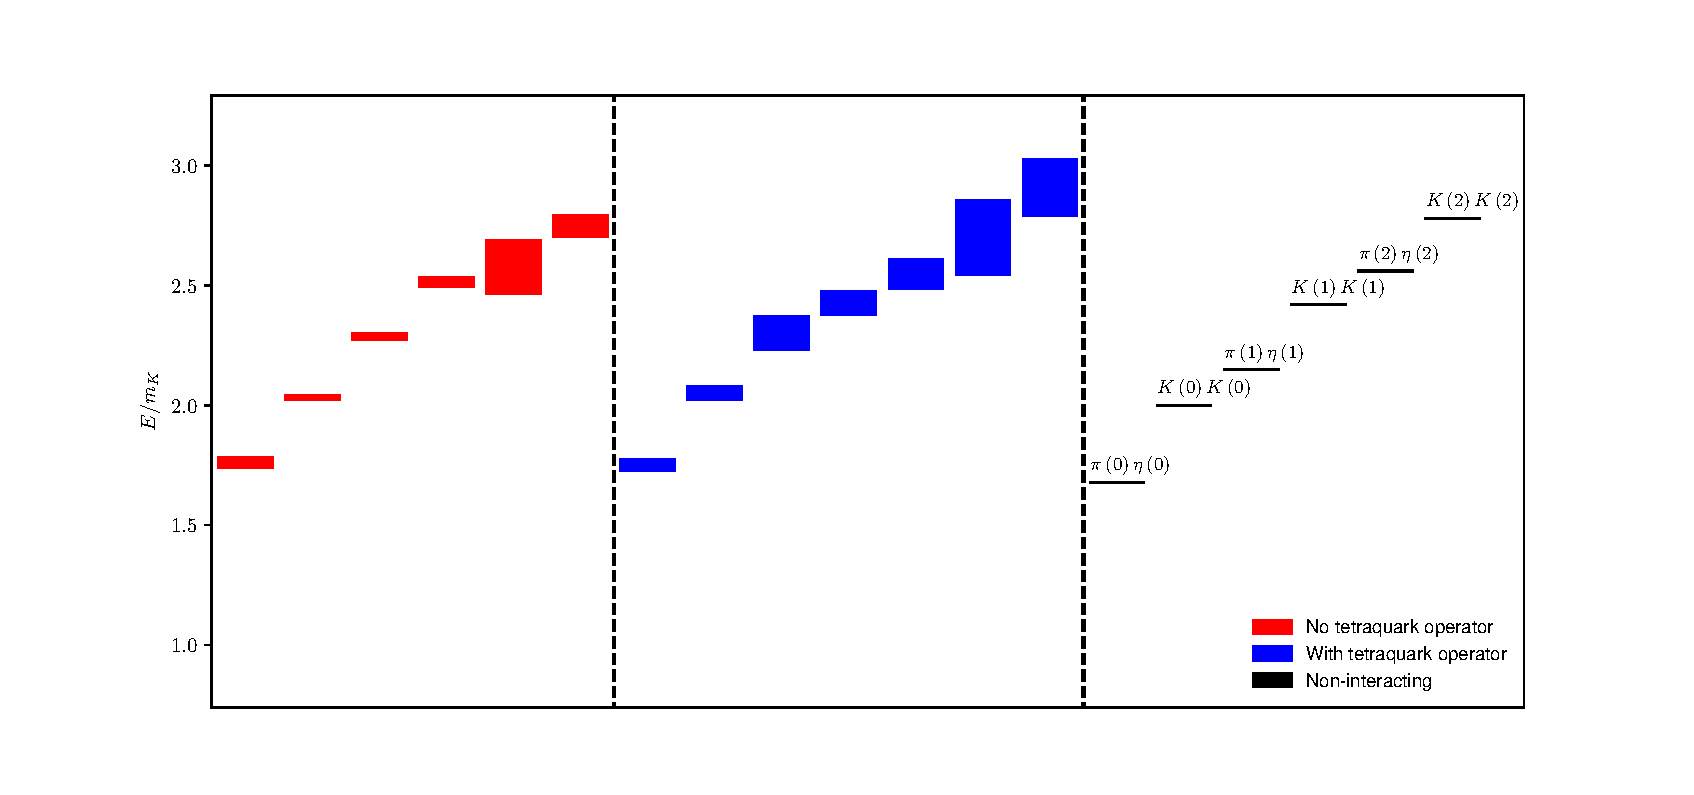
\includegraphics[scale=0.7]{figures/a1gm_staircase.pdf}
  \caption{The first six and seven levels of the spectrum in the $a_0(980)$ at-rest symmetry channel. On the left: the spectrum obtained using a basis with no tetraquark operators. In the middle: the spectrum obtained using one tetraquark operator. On the right: non-interacting levels shown for reference, where $(\boldsymbol{d}^2)$ denotes particles with squared momentum $(2\pi\boldsymbol{d}/L)^2$.}\label{fig:a0_spectrum}
\end{figure}